\chapter{Naive Bayes Nearest Neighbor} % (fold)
\label{cha:naive_bayes_nearest_neighbor}

The focus of this thesis is on the Naive Bayes Nearest Neighbor (NBNN) image classification method, first presented by Boiman \emph{et al.} \cite{boiman2008defense}. In this section the theory behind the method, its sources and its later adaptations will be discussed.

\section{$k$-Nearest Neighbor Classification} % (fold)
\label{sub:_k_nearest_neighbor}

The $k$-Nearest-Neighbor algorithm is one of the earliest approaches for classification in machine learning. Given a set of items $n \in \mathcal{N}$, labeled with a designated number of classes $c_n \in \mathcal{C}$, an unlabeled query item $q$ and a distance measure to calculate pairwise differences between items $d(x_1\|x_2)$, the nearest neighbors of $q$ are the $k$ items in $\mathcal{N}$ for which $d(q\|n)$ is lowest. In turn, sets $\text{NN}_c(q)$ contain those nearest neighbors of $q$ that belong to class $c$. This way, $k$NN classification comes down to
\begin{align}
    \hat c_q &= \argmax_c |\text{NN}_c(q)|,
\end{align}
being the class of which the most items are within the $k$ nearest neighbors of $q$.

In contrast to other classification algorithms, $k$NN is relatively simple. It does not require any training to make a model from the labeled images. The algorithm only estimates the probability density of the classes locally, within $k$, which means it does not assume a global probability density distribution underneath the data, which makes it a model-free non-linear classifier.

\section{Naive Bayes Classification} % (fold)
\label{sub:NB}

Naive Bayes is another rather simple classification algorithm, which is based on the idea that a simplification of Bayes' Theorem can be made using the assumption that all features $d_{n,i} \in \mathcal{D}_n$ of an item $n$ appear conditionally independent of each other. This means that for all images, all classes $c$ and all non-equal features $d_{n,i} \neq d_{n,j}$, 
\begin{align}
    p(d_{n,i} | c_n, d_{n,j}) = p(d_{n,i}|c_n)
\end{align}
is assumed.
If Bayes' Theorem is modeled to predict the probability of a class $c$ of an item $q$, we can say
\begin{align}
    \label{eq:bayes}
    p(c|q)      &= \frac{p(q|c)\,p(c)}{p(q)}\\
                &\propto p(q|c)\,p(c),
\end{align}
because the probability is to be compared among all classes $\mathcal{C}$, for the same item $q$, which makes $p(q)$ constant. Furthermore, if $q$ is represented by $m$ features $d_q$, \eqref{eq:bayes} can be rewritten as
\begin{equation}
    p(c|d_{q,1},\dotsc,d_{q,m}) = p(d_{q,1}, \dotsc,d_{q,m}|c)\,p(c),
\end{equation}
which is equivalent to the joint probability
\begin{align}\begin{split}
    p(c|d_{q,1},\dotsc,d_{q,m}) &\propto p(c,d_{q,1}, \dotsc,d_{q,m})\\
        &\propto p(c)\,p(d_{q,1}|c)\, p(d_{q,2}|c,d_{q,1}), \dotsc,p(d_{q,m}|c,d_{q,1},d_{q,2},\dotsc,\\&\quad d_{q,m-1}).
    \end{split} 
\end{align}
By the conditional independence assumption made above, this can be reduced into
\begin{equation}
    p(c|q) \propto p(c)\prod_{i=1}^m p(d_{q,i}|c).
\end{equation}
With this equation, a decision rule can be made as follows
\begin{equation} \label{eq:map}
    \hat c_q = \argmax_c \frac{1}{m}\,p(c)\prod_{i=1}^m p(d_{q,i}|c),
\end{equation}
which is called a maximum a-posteriori (MAP) classifier. In this formulation of a classification problem, a probability density estimation is needed to model all features. All kinds of distributions can be used for this.

\section{Boiman's NBNN} % (fold)
\label{sub:boiman_s_nbnn}
Boiman \emph{et al.} \cite{boiman2008defense} coined the term Naive Bayes Nearest Neighbor (NBNN) for their image classification algorithm that used a combination of Nearest-Neighbor (NN) and Naive Bayes to classify images in a multi-class setting. The approach works well because of the model-free character of the approach, which means no tuning of model-parameters is required. This makes it easy to use the method on a problem with a large number of classes, while parametric methods typically model multi-class problems as multiple 2-class problems. It also means that the risk of overfitting is smaller because there are no model parameters to be tuned. The only parameters are in the (type and amount of) features, which is the same for other classification methods. The authors achieved results competitive to the state of the art Bag of Features (BoF) methods because the method benefits from two requirements it meets: (\emph{i}) Avoiding feature quantization and (\emph{ii}) the use of image-to-class distance instead of image-to-image distances. They theorize that earlier attempts to use NN \cite{berg2005shape, zhang2006svm} for image classification failed because these do not meet both requirements.

\begin{figure}[hbt]
    \centering
    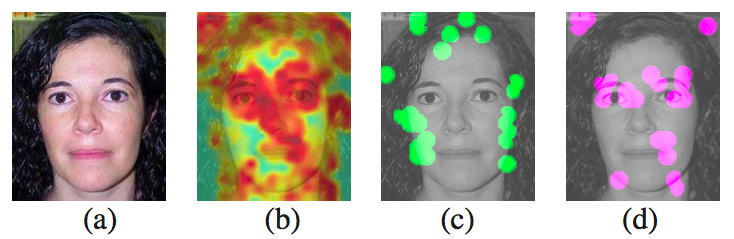
\includegraphics[width=0.9\textwidth]{QuantizationError}
    \caption{Visualization of the quantization error. (a) An image from the ``face'' class in Caltech101. \cite{caltech101} (b) ``Quantization error of densely sampled SIFT descriptors using a large codebook of Caltech101. Red = high error; Blue = low error. The most informative descriptors (eye, nose, etc.) have the highest quantization error.'' (c) ``Green marks the 8\% of the descriptors in the image that are most frequent in the database (simple edges).'' (d) ``Magenta marks the 8\% of the descriptors in the image that are least frequent in the database (mostly facial features)''. Taken from Boiman \emph{et al.} \cite{boiman2008defense}.}
    \label{fig:quantization_error}
\end{figure}

Feature quantization is a means of creating compact image descriptions, such as the ones used in the BoF methods. In BoF, all descriptors of an image are clustered into visual words, and histograms are constructed counting the occurrence of each word in an image. Image matching is based on comparing these histograms. Quantization is harmful for a nearest neighbor approach because the most informative descriptors get the highest quantization error while being necessary for finding nearest neighbors. This becomes clear when the observation is made that for a descriptor to be more informative, it should appear only at certain circumstances, ideally only in images of one class. They should be fairly well recognizable among other descriptors, and therefore they tend to be outliers in descriptor space. When quantizing, these descriptors will mostly be incorporated into visual words that are rather unlike these descriptors, resulting in a large quantization error. In Figure~\ref{fig:quantization_error}, the effects of this are illustrated.

In learning-based methods, like SVM, this quantization error is outweighed by the benefit of dimensionality reduction which allows training on a large data set. Furthermore, the problem itself is mitigated in BoF methods. The learning phase in these methods makes sure that only descriptors that are good predictors, regardless of their quantization error, are considered in the test phase. Because NBNN does not have a learning phase nor dimensionality reduction, it has to use every single descriptor of each image to perform NN on to avoid the quantization error.

Codebook are based on image-to-image distances to create decision boundaries. For each image in the training set, a histogram of visual words is built, based on the features that appear in the image, and are matched with the visual words that resulted from quantizing all training features. 
In a nearest neighbor approach, image-to-image distances do not enable much generalization, as no inference is done from the training images and their features. This would mean only test images close to known images will be classified correctly. Therefore, image-to-class distances should be used. While an image might be far removed from all others of a certain class, the individual features might all be close to features of different images of this class, making the image-to-image distances to a class large, but the image-to-class distance short \cite{wang2009learning}. Figure~\ref{fig:im2im_vs_im2cl} shows the difference between image-to-image distance and image-to-class distance.

\begin{figure}[hbt]
    \centering
    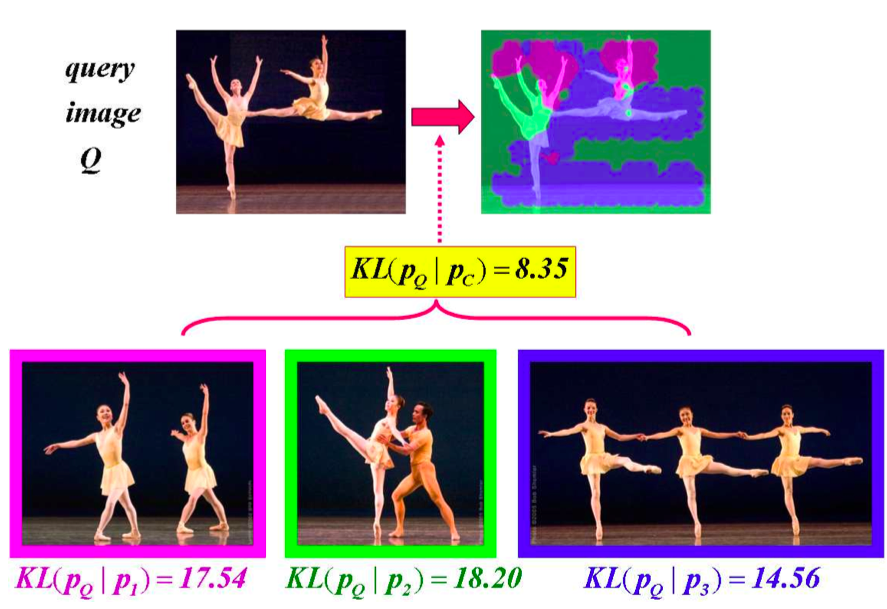
\includegraphics[width=0.9\textwidth]{Im2imVsIm2cl}
    \caption{Image-to-class distance versus image-to-image distance. Given three labeled images of the ``ballet''-class (bottom row), and a query image (top left). Even though the ``Query-to-image'' distance is large to each individual labeled image, represented by the KL-divergences, the ``Query-to-class'' distance is small. The top right image shows the query image, with each descriptor having the color of the labeled image which gave it the highest descriptor likelihood. It shows that this query configuration is more likely given the three images, than each individual image separately. Taken from Boiman \emph{et al.} \cite{boiman2008defense}, original images from Irani \& Boiman \cite{irani2006similarity}.}
    \label{fig:im2im_vs_im2cl}
\end{figure}

Using the main points of no quantization and image-to-class distances, $k$-nearest neighbor can be performed for individual features, per class. Note that in this way, each individual feature could be classified as its NN, but a second step is required to classify images as a whole. Therefore the set of individual distances is used as the input of a Naive Bayes classifier.

The NBNN decision rule is defined under the Naive Bayes assumption of Section~\ref{sub:NB}. The MAP classifier from Equation \eqref{eq:map}, when assuming uniform priors $p(c)$ over all classes, simplifies to Maximum Likelihood (ML) classifier 
\begin{align}
    \hat c &= \argmax_c \frac{1}{m}\prod_{i=1}^{m} p(d_{q,i}|c)\\
           &\propto \argmax_c \frac{1}{n}\sum_{i=1}^{n} \log p(d_{q,i}|c),
\end{align}
Where the last formulation as a sum of log-probabilities is used in practice to compensate for the low probabilities typical for this classifier, which may cause rounding errors in computer applications.

Using the notion that NN classification tends to the Bayes optimal classifier when the sample size tends to infinity\cite{boiman2008defense, cover1967nearest}, dense sampling can be used to get a high number of descriptors per class from the training set $Z = |\mathcal{D}_c|$. The class conditional probability of a feature $p(d_q|c)$ can be modeled using Parzen likelihood estimation, where
\begin{equation} \label{eq:parzen}
    \hat p(d_q|c) = \frac{1}{Z}\sum_{j=1}^Z K(d_q-d_{c,j}).
\end{equation}
Parzen kernel function $K(\cdot)$, typically Gaussian, defines the distance between query descriptor $d_{q}$ and labeled descriptor $d_{c}$. When $Z$ goes to infinity, $\hat p(f|c)$ approaches $p(f|c)$. 

This approach entails calculating the distance of $d$ to all $Z$ descriptors of each class, which would be very costly. Because only a small minority of the descriptors can be expected to be significantly close to $d_q$, taking into account only the nearest descriptors is a safe approximation, which enables using nearest neighbors (NN) to find these descriptors. Even more so, Boiman shows that the performance loss of taking only the 1 nearest neighbor is very small. Because of this the Parzen estimate of $d_q$ to class $c$ reduces to the distance of $d_q$ to its nearest neighbor in $c$: $\|d_q - \text{NN}_c(d_q)\|^2$, resulting in the following log likelihood and classifier: 
\begin{align}
    \label{eq:nbnnloglikelihood}
    \log P(q|c) &\propto -\sum_{i=1}^m \|d_{q,i} - \text{NN}_c(d_{q,i})\|^2 \\
    \label{eq:nbnnclass}
    \hat c      &= \argmin_c \sum_{i=1}^m \|d_{q,i} - \text{NN}_c(d_{q,i})\|^2
\end{align}

Now, classification boils down to calculating descriptors for all images in each class and for the query image, estimating the nearest neighbor of each query descriptor for each class, calculating the sum of distances for each class for the query image and selecting the lowest distance. This approach is both very simple and intuitive. It also enables use of different kinds and combinations of descriptors.

% subsection boiman_s_nbnn (end)


\section{Limitations and Extensions} % (fold)
\label{sub:limitations_and_extensions}

Even though the algorithm of Boiman \emph{et al.} \cite{boiman2008defense} is very simple and requires no learning phase, it does have scalability issues because of its dependence on having as many individual descriptors as possible. Because all densely computed descriptors for each image in the training set have to be stored, and the nearest neighbor for each descriptor of each query image on each class has to be found, the time and memory usage is much higher than for example BoF methods, which use a more compact representation of images. Calculating NN can be sped up by using sophisticated approximations of the Nearest Neighbor algorithm, such as FLANN \cite{muja2009fast}, which uses randomized kd-trees to provide a quick search in a k-dimensional search space. This relieves some time issue, but is not a remedy for the memory issues.

% section limitations_and_extensions (end)

\subsection{Local NBNN} % (fold)
\label{sec:local_nbnn}

An adaptation of NBNN by McCann \& Lowe called local NBNN (LNBNN) \cite{mccann2012local} has another approach to solve some of the limitations of the original algorithm. Their main idea is that it is not necessary to find a descriptor's nearest neighbor in each class separately, but that is sufficient to find the $k$ nearest neighbors over all classes. It will perform better, in fact. See Figure~\ref{fig:lnbnn} for a visualization of the conceptual difference.

This simplification of the basic query implies a more efficient algorithm, because it is much faster to search for $k$ nearest neighbors in one collection, than to search for 1 NN for each class, even when $k$ is much larger than the number of classes.

Besides the time-complexity benefit, LNBNN also enhances the results of NBNN. Because only the $k$NN are taken into account, it might well be that not all classes will be involved for each descriptor in an image. In the original NBNN, these distances would still be taken into account, lowering the chance of the class to get the highest probability for the image by a possibly large amount. LNBNN takes the $k+1$-th distance for these classes, making this effect much less significant. Liu \emph{et al.} \cite{liu2011defense} have hypothesized that in a sparse manifold space, such as the descriptor space, larger distances give a much worse estimate of membership to a class. This might be the cause for the improved results that LNBNN gets compared to Boiman's NBNN. Another argument is that each descriptor should only add bits of evidence to the probability of an object's class. It should not lower this probability. Otherwise the influence of background clutter could be too large.

LNBNN will be used as a basis for the object detection algorithm, because it is an efficient variant of NBNN, and extends to the $k>1$ case, which proved to be important in the detection case.

\begin{figure}[hbt]
    \centering
    \begin{subfigure}[b]{0.60\textwidth}
        \centering
        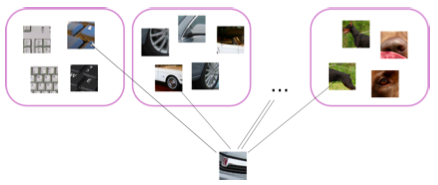
\includegraphics[width=\textwidth]{LNBNNa}
        \caption{The original NBNN asks, ``Does this descriptor look like a keyboard? a car? \ldots a dog''}
        \label{fig:lnbnna}
    \end{subfigure}%
    ~ %add desired spacing between images, e. g. ~, \quad, \qquad etc.
      %(or a blank line to force the subfigure onto a new line)
    \begin{subfigure}[b]{0.30\textwidth}
        \centering
        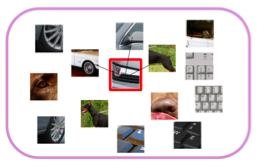
\includegraphics[width=\textwidth]{LNBNNb}
        \caption{Local NBNN asks, ``What does this descriptor look like?''}
        \label{fig:lnbnnb}
    \end{subfigure}%
    \caption{Difference in conceptual approach of regular NBNN and Local NBNN. Taken from McCann \& Lowe \cite{mccann2012local}.}
    \label{fig:lnbnn}
\end{figure}

% subsection local_nbnn (end)


% section naive_bayes_nearest_neighbor (end)